%!TEX ROOT=../emnlp2023.tex

\section{Introduction}
\label{sec:introduction}
We release pipeline for fact-checking claims using evidence retrieved from the web consisting of two modules -- a \textit{retriever}, which picks the most relevant sources among the available knowledge store\footnote{Due to the pre-retrieval step that was used to generate knowledge stores, our \say{retriever} module could more conventionally be referred to as a \say{reranker}, which we refrain from, to avoid confusion with reranking steps it uses as a subroutine.} and an \textit{evidence \& label generator} which generates evidence for the claim using these sources, as well as its veracity label. 

Our pipeline is a variant of the popular Retrieval-augmented Generation (RAG) scheme~\cite{rag}, making it easy to re-implement using established frameworks such as Langchain, Haystack, or our attached Python codebase for future research or to use as a baseline.

This paper describes our pipeline and the decisions taken at each module, achieving a simple yet efficient RAG scheme that improves dramatically across the board over the baseline system from~\cite{averitec2024}, and scores third in the \averitec{} leaderboard as of August 2024, with an \averitec{} score of 50.4\%.

% show figures/pipeline.png
\begin{figure}[h]
    \centering
    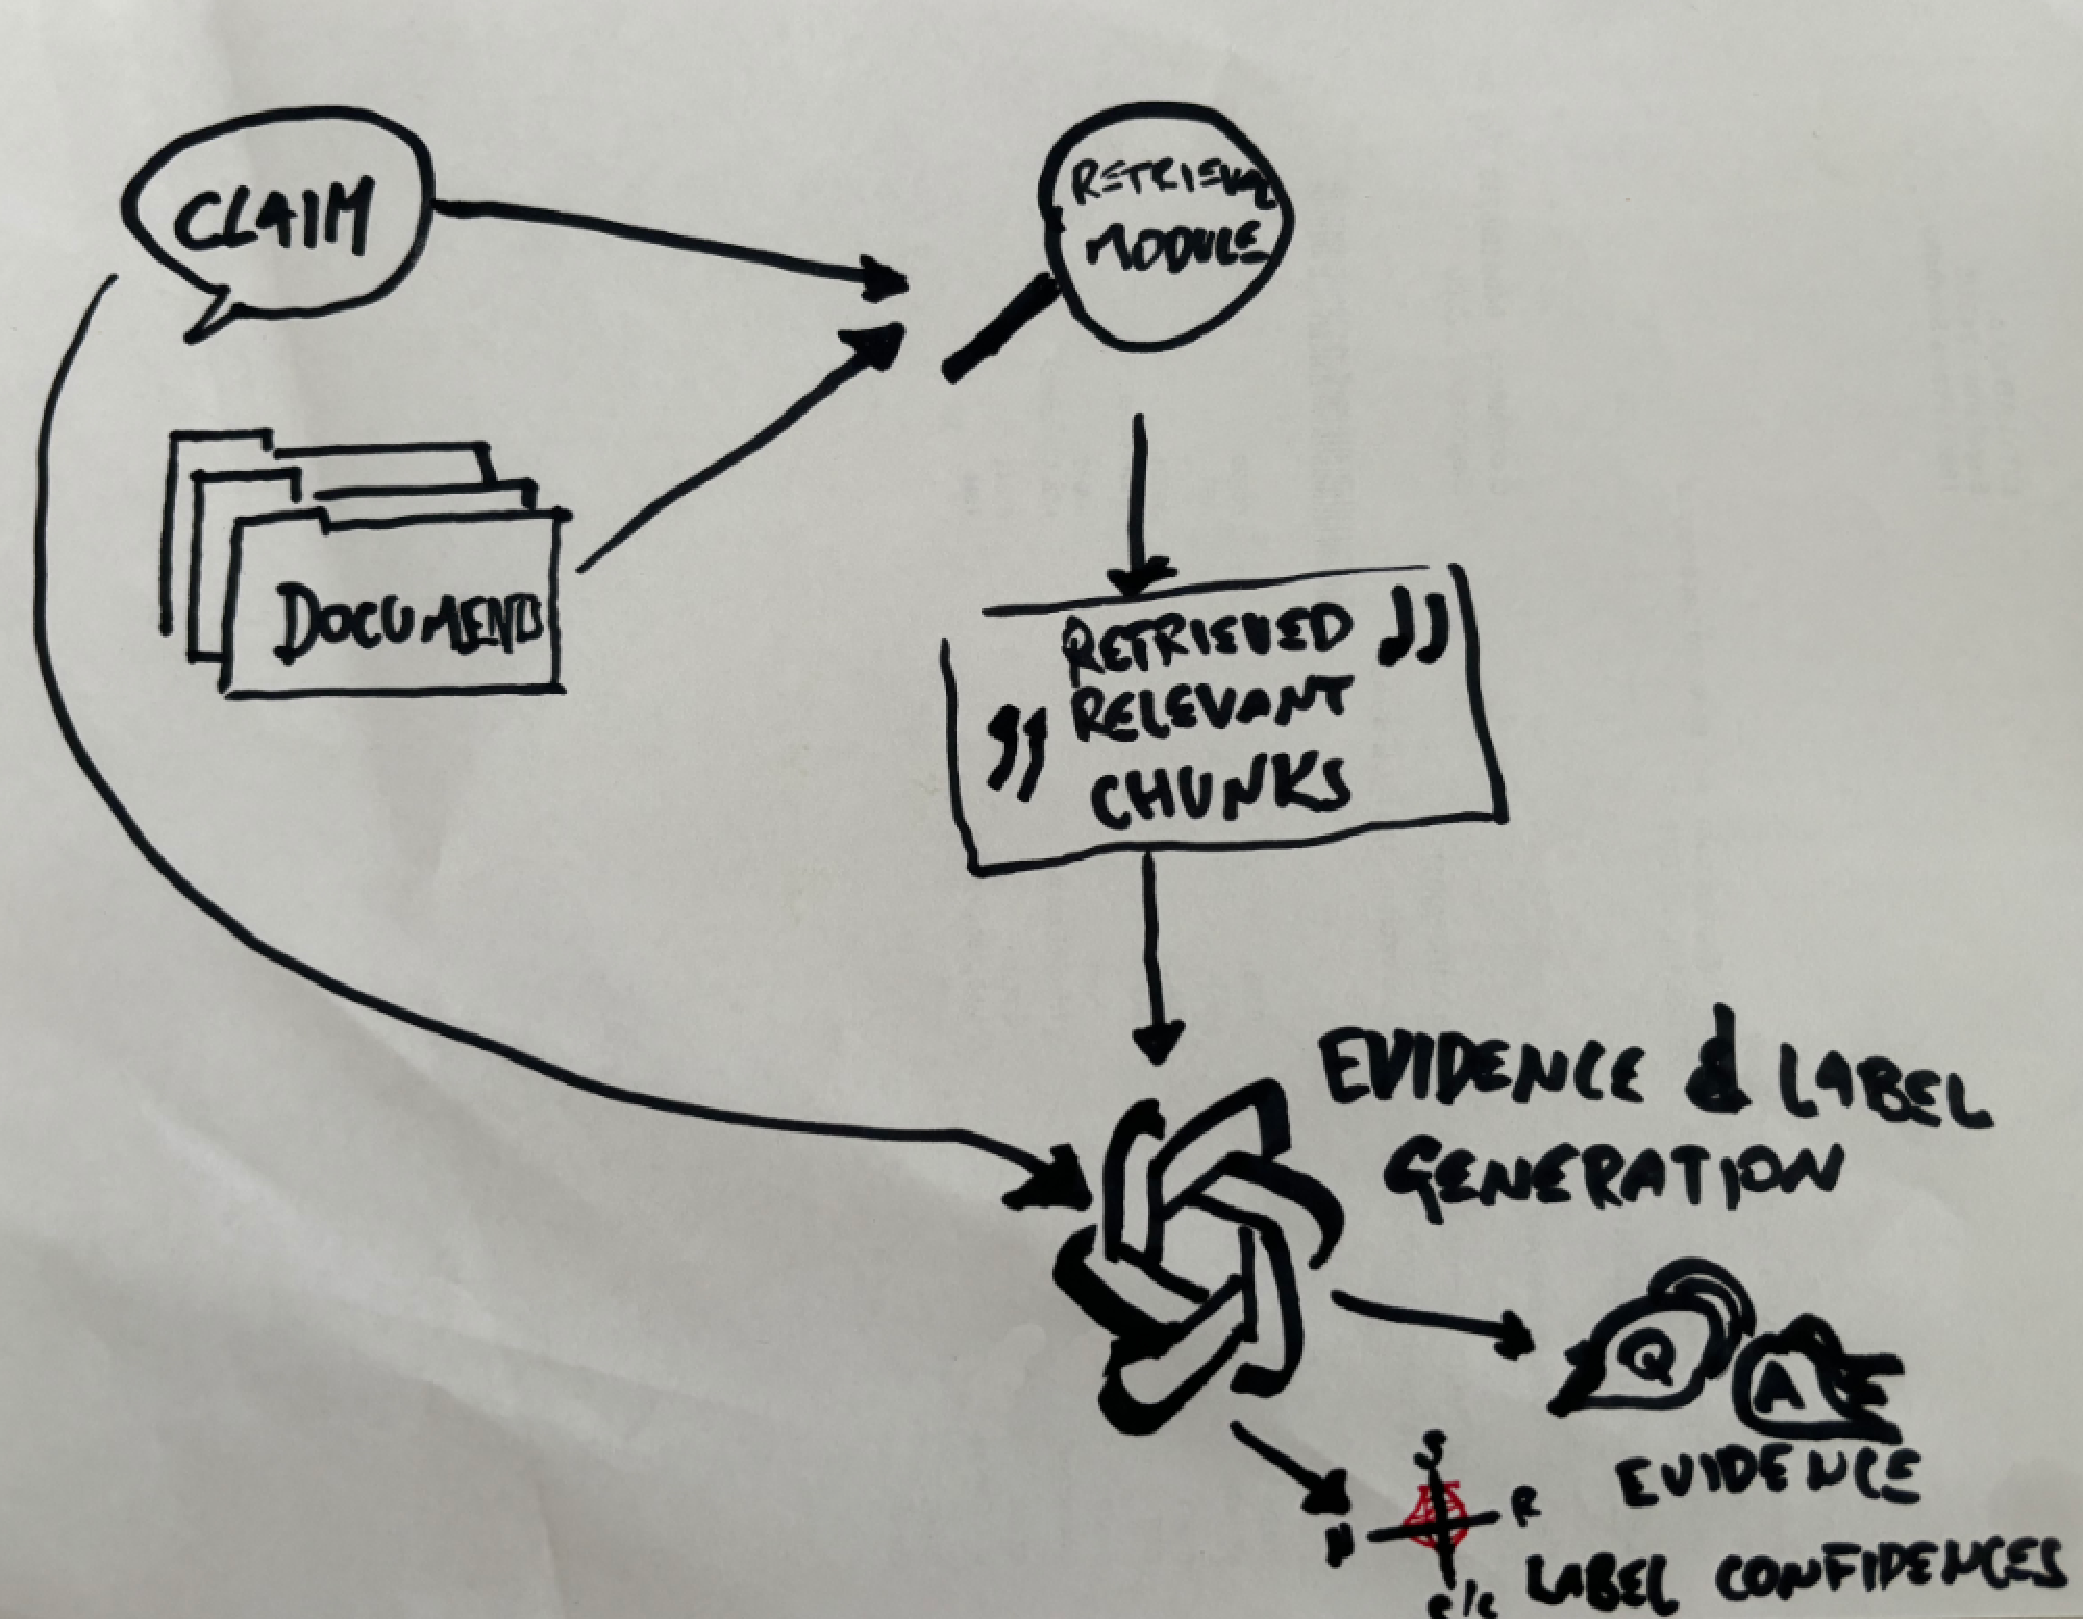
\includegraphics[width=0.47\textwidth]{figures/pipeline.pdf}
    \caption{Our pipeline}
    \label{fig:pipeline}
\end{figure}

\section{Related work}
\label{sec:relwork}
\label{avscore}
\begin{enumerate}
    \item \textbf{\averitec{} shared task}~\cite{averitec2024} releases the dataset of real-world fact-checked claims, annotated with evidence available at the date the claim was made.
    
    It proposes the \textbf{\averitec{} Score} -- a method of unsupervised scoring of fact-checking pipeline against this dataset using Hungarian METEOR score (matching the evidence questions (Q) or the whole evidence (Q+A)), and then counting the proportion of claims with accurate label and sound evidence at the same time (using a threshold for Hu-METEOR such as 0.25) among all claims in the dataset, giving an estimate on \say{how often the whole fact-checking pipeline succeeds end to end}.

    The provided \textbf{baseline} is a pipeline of search query generation, API search (producing a knowledge store), sentence retrieval, Question-and-answer (QA) generation, QA reranking, QA-wise claim classification and label aggregation, achieving an overall \averitec{} score of 11\%.  
    \item \textbf{FEVER Shared Task}~\cite{thorne-etal-2018-fact}, a predecessor to the \averitec{} worked with a similar dataset engineered on top of the enclosed domain Wikipedic data rather than real-world fact-checks -- its top-ranking solutions used a simpler pipeline of Document Retrieval, Sentence Reranking and Natural Language Inference, improving its modules in a decoupled manner and scoring well above 60\% in a similarly computed FEVER score~\cite{thorne-etal-2018-fever} on this data.
    \item \textbf{Our previous research} on fact-checking pipelines~\cite{Ullrich2023,drchal2023pipelinedatasetgenerationautomated} using data similar to FEVER and \averitec{} shows significant superiority of fact-checking pipelines that \textbf{retrieve the whole documents} for the inference step, rather than retrieving out-of-context sentences.
    \item \textbf{Retrieval-Augmented Generation (RAG) for Knowledge-Intensive Tasks}~\cite{rag} takes this a step further, leveraging Large Language Model (LLM) for the task, providing it the whole text of retrieved documents (each a chunk of Wikipedia) and simply instructing it to predict the evidence and label on top of it, achieving results within 4.3\% from the FEVER state of the art by the time of its publication (December 2020) \textit{without} engineering a custom pipeline for the task.
\end{enumerate}

